\documentclass{standalone}
\usepackage{ tikz }
\usepackage{ xparse }
\input{macros/all}

\begin{document}
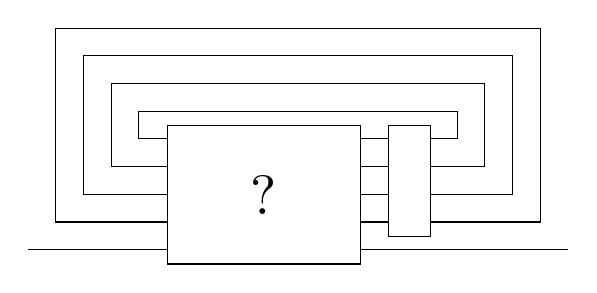
\begin{tikzpicture}[yscale=-1,x=1em,y=1em] \draw
    (0,5) -- (5,5)
    (5,4) -- (1,4) -- (1,-3) -- (18.5,-3) -- (18.5,4) -- (14.5,4)
    (14.5, 3) -- (17.5,3) -- (17.5, -2) -- (2,-2) -- (2,3) -- (5,3)
    (14.5,2) -- (16.5, 2) -- (16.5,-1) -- (3,-1) -- (3,2) -- (5, 2)
    (14.5,1) -- (15.5,1) -- (15.5,0) -- (4,0) -- (4,1) -- (5,1)
    
    % shuffle to edges

    (12,5) -- (19.5,5)
    (12,4) -- (13,4)
    (12,3) -- (13,3)
    (12,2) -- (13,2)
    (12,1) -- (13,1)
    
    node[draw,minimum width=7em,minimum height=5em,anchor=north west] at (5,0.5){\scalebox{2}{$?$}}
    node[draw, minimum width = 1.5em, minimum height = 4em, anchor=north west] at (13,0.5){\scalebox{0.75}{\rotatebox[origin=c]{-90}{$\stackfun$}}}

;\end{tikzpicture}
\end{document}